\chapter{Theoretical Background}
\label{chap:background}

This chapter provides the theoretical foundations for this thesis, covering three main areas. Section~\ref{sec:sar_forest} examines SAR remote sensing for forest parameter estimation, including the physical basis of radar-vegetation interactions and existing approaches for height and species extraction. Section~\ref{sec:mtl_rs} reviews multitask learning principles and their application in remote sensing contexts. Section~\ref{sec:datasets} discusses dataset availability for forest monitoring research and the challenges of obtaining multitask annotations.

\section{SAR Imagery for Forest Parameter Estimation}
\label{sec:sar_forest}

Synthetic Aperture Radar has become a valuable tool for forest monitoring because it offers capabilities that optical sensors cannot match. The main advantage is that SAR actively transmits microwave pulses and records the backscattered signal, which means it can acquire imagery regardless of sunlight or weather conditions. This all-weather, day-and-night capability is especially useful for monitoring forests in regions with frequent cloud cover, where optical data is often unavailable \cite{moreira_tutorial_2013}.

How SAR interacts with forest canopies reveals information about vegetation structure that optical sensors miss. The key factor is wavelength, which determines how deeply the signal penetrates: X-band signals interact mainly with leaves and small branches at the canopy surface, C-band (used by Sentinel-1) penetrates into the upper canopy structure, while L-band and P-band wavelengths can reach tree trunks and even the ground surface. This penetration capability allows SAR to sense vertical forest structure, making it sensitive to parameters like canopy height.

Research has demonstrated the potential of SAR data for forest canopy height estimation. ~\cite{li_high-resolution_2020} showed that coupling ICESat-2 LiDAR with Sentinel-1, Sentinel-2 and Landsat-8 data achieved correlation coefficients of 0.78 for canopy height prediction, with the addition of Sentinel-1 backscattering coefficients contributing positively to model performance. Similarly, ~\cite{wei_forest_2024} found that synergizing ICESat-2, Sentinel-1, Sentinel-2 and topographic information using Random Forest achieved RMSE values of 3.15--3.37~m for different forest types in China. \cite{srivastava_joint_2017} demonstrated joint estimation of multiple forest parameters from SAR data, showing that coupled predictions can improve accuracy through shared feature learning. The VH and VV polarization channels from Sentinel-1 were validated as important predictors, with cross-polarized backscatter (VH) showing stronger sensitivity to vegetation structure due to its response to volume scattering.

Deep learning approaches have recently advanced canopy height estimation capabilities. \cite{lang_high-resolution_2023} developed a probabilistic deep learning model that fused sparse GEDI LiDAR data with Sentinel-2 optical images, producing global canopy height maps at 10~m resolution with RMSE of 7.9~m. \cite{castro_deep_2024} found that combining seasonal Sentinel-1 and optical features with PALSAR data yielded $R^2$ of 0.72 and RMSE of 3.43~m for northern forests, noting that SAR data provides valuable structural insights complementary to optical spectral information. For SAR-specific approaches, \cite{mahesh_forest_2024} investigated forest height estimation using TanDEM-X InSAR features with deep learning, demonstrating that interferometric coherence and backscatter can be combined in convolutional neural networks for height prediction, achieving RMSE of 6.12~m with volumetric decorrelation as the primary input feature. \cite{mahesh_deep_2023} further explored deep learning for forest canopy height estimation from SAR, showing that convolutional architectures can extract height-relevant features from InSAR products and single-look complex SAR images. Recent work has also explored fusing physical models with deep learning. \cite{wei_forest_2024} proposed using InSAR coherence as an indicator for forest canopy height estimation, establishing relationships between coherence stability and vegetation structure. \cite{mahesh_better_2025} developed CoHNet, an end-to-end framework that fuses physical models with deep learning by optimizing volume decorrelation through a physics-aware training loss, demonstrating that incorporating physical constraints improves forest height estimation accuracy compared to purely data-driven methods.

For tree species classification from SAR, research has shown that texture features, temporal patterns, and polarimetric decomposition products provide discriminative information. The TreeSatAI benchmark \cite{ahlswede_treesatai_2023} demonstrated that Sentinel-1 data contributes to species classification when combined with optical imagery, though optical sensors typically achieve higher accuracy when used alone. \cite{dostalova_european_2021} achieved European-wide forest classification using Sentinel-1 data, demonstrating the potential of C-band SAR for vegetation type discrimination. \cite{udali_assessing_2021} assessed forest type and tree species classification using Sentinel-1 C-band SAR data in southern Sweden, finding that backscatter coefficients from VV and VH polarizations combined with temporal features achieved classification accuracies up to 85\% for dominant species. More recently, \cite{grace_tree_2024} explored tree species classification using machine learning and 3D tomographic SAR data in northern Europe, demonstrating that tomographic features extracted from multi-baseline SAR acquisitions provide additional discriminative power for species identification.

The C-band wavelength of Sentinel-1 presents both opportunities and challenges for forest applications. The free availability, global coverage, and frequent revisit make Sentinel-1 data accessible for operational applications in a way that commercial SAR sensors are not. However, C-band has limited penetration into dense forest canopies compared to longer wavelength systems like L-band ALOS-2 PALSAR, which affects sensitivity to height in mature forests with closed canopies. Despite these limitations, C-band SAR has shown useful correlations with canopy height, particularly when temporal features or texture information are exploited.

The reason for investigating SAR-only approaches relates to operational constraints. While optical-SAR fusion generally improves model performance, the requirement for cloud-free optical imagery limits how frequently predictions can be made. Approximately 67\% of Earth's surface is covered by clouds at any given time, and in tropical forests where cloud cover persists throughout much of the year, waiting for clear optical scenes may delay monitoring by weeks or months. \cite{wu_segcr_2025} demonstrated that semantic change detection can be performed effectively using SAR data alone, highlighting the value of all-weather monitoring capabilities for time-sensitive applications. A robust SAR-based approach would enable continuous monitoring regardless of atmospheric conditions, supporting applications in forest change detection, degradation monitoring, and inventory updating where timeliness is important. Furthermore, developing SAR-only methods has value for understanding what information SAR actually provides about forests. When SAR is always combined with optical data, it becomes difficult to isolate the contribution of radar features to the prediction. By investigating SAR-only models, this research aims to clarify the extent to which structural information in radar backscatter can support forest parameter extraction.

\section{Multitask Learning in Remote Sensing}
\label{sec:mtl_rs}

Multitask learning is a machine learning approach where a single model learns to perform multiple related tasks at the same time, using shared representations to boost performance across all tasks. The core idea is straightforward: when tasks are related, they can benefit from learning common features together rather than separately. This joint learning acts as a form of regularization, helping the model avoid overfitting to task-specific noise and improving its ability to generalize.

\subsection{Deep Learning Architectures for Multitask Learning}

\cite{vandenhende_multi-task_2021} provided a comprehensive survey of MTL approaches for dense prediction tasks in computer vision, establishing a taxonomy of architectural strategies. Figure~\ref{fig:mtl-basics} illustrates this taxonomy, showing how different MTL architectures organize the flow of information between tasks. The survey identifies two fundamental paradigms for parameter sharing in deep multitask networks: hard parameter sharing and soft parameter sharing.

\begin{figure}[htbp]
\centering
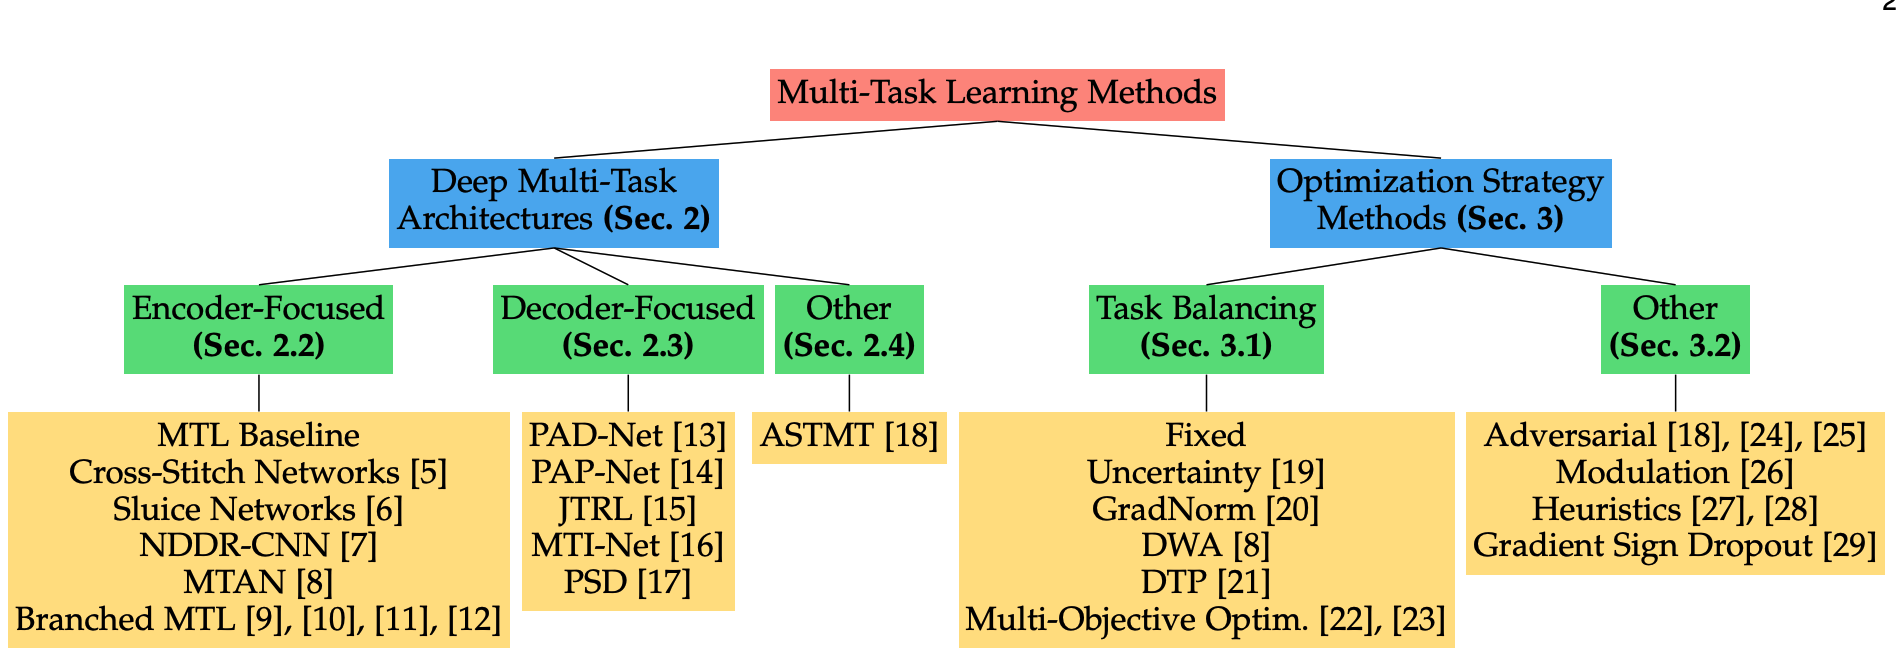
\includegraphics[width=0.9\textwidth]{img/mtl-basics.png}
\caption{A taxonomy of deep learning approaches for jointly solving multiple dense prediction tasks. The figure shows different architectural strategies including hard parameter sharing (shared encoder with task-specific decoders), soft parameter sharing (task-specific networks with cross-connections), and attention-based approaches. Adapted from \cite{vandenhende_multi-task_2021}.}
\label{fig:mtl-basics}
\end{figure}

\textbf{Hard parameter sharing} is the most common approach. Here, all tasks share the same encoder network that extracts features from the input, while each task gets its own decoder (or output head) to produce task-specific predictions. This setup forces the shared encoder to learn representations that are useful for all tasks simultaneously. The main advantage is efficiency: you only need one encoder instead of multiple separate networks. The challenge is that the shared encoder must balance the needs of different tasks, which can be difficult when tasks have conflicting requirements.

\textbf{Soft parameter sharing} takes a different approach. Each task has its own network with its own parameters, but these networks communicate with each other through specialized connection mechanisms. This allows tasks to share information selectively rather than forcing everything through a single shared encoder. \cite{misra_cross-stitch_2016} introduced cross-stitch networks, which use learnable linear combinations to mix activations between task-specific networks at multiple layers. The cross-stitch units learn how much information each task should receive from the other tasks' representations, enabling flexible sharing patterns that can adapt during training. The Multi-Task Attention Network (MTAN) uses attention mechanisms to learn task-specific feature-level attention. Each task has its own attention network that selectively focuses on relevant features from a shared backbone, allowing the model to automatically determine which features are important for each task.

The choice between hard and soft parameter sharing involves trade-offs. Hard sharing is more parameter-efficient and provides stronger regularization, but it can suffer when tasks are only weakly related or have conflicting optimization requirements. Soft sharing offers more flexibility and can better handle diverse tasks, but requires more parameters and careful design of the cross-task communication mechanisms. The optimal choice depends on task relatedness, available training data, and computational constraints.

\subsection{Multitask Learning for Forest Monitoring}

In remote sensing, multitask learning has been applied to various forest monitoring problems, though most work focuses on optical imagery. \cite{plotnikov_multitask_2025} explored multitask learning for estimating primary forest characteristics using Sentinel-2 data, demonstrating that jointly predicting multiple forest attributes (such as tree height, diameter, and basal area) from optical imagery improves estimation accuracy compared to single-task models. Their approach used a shared convolutional encoder with task-specific regression heads, showing that structural forest parameters share underlying spectral patterns that can be exploited through joint learning.

\cite{cui_mtscd-net_2023} proposed MTSCD-Net, a network based on multitask learning for semantic change detection of bitemporal remote sensing images. The architecture combines binary change detection (identifying where changes occurred) with semantic change detection (classifying the type of change) as complementary tasks. \cite{tao_multi-task_2025} developed a multitask learning framework with enhanced cross-level semantic consistency for multi-level land cover classification. Their approach addresses the hierarchical nature of land cover classification systems. By jointly learning classifications at multiple hierarchical levels and enforcing semantic consistency between levels, the model achieves improved accuracy at both coarse and fine scales compared to training separate classifiers for each level. Recent advances in multitask learning architectures have explored state-space models, with \cite{shen_learning_2025} demonstrating that Mamba-based architectures can effectively handle multiple dense prediction tasks in remote sensing through efficient long-range dependency modeling. \cite{liu_associatively_2022} proposed associative learning mechanisms that enable tasks to share knowledge more effectively through learned task relationships rather than fixed architectural constraints.

For hyperspectral imagery, \cite{chhapariya_multitask_2024} developed a multitask deep learning model for simultaneous classification and regression of hyperspectral images, applying it to large-scale datasets. Figure~\ref{fig:mtl-rs-model} shows their proposed framework. The architecture consists of a shared encoder based on ResNet with Dense Atrous Spatial Pyramid Pooling (ASPP), followed by spectral-spatial attention blocks and task-specific decoders. Each output has its own loss criterion: Cross-Entropy (CE) for classification and Mean Absolute Error (MAE) for regression. The model addresses class imbalance through cost-sensitive learning and focal loss, while balancing multiple task objectives using uncertainty weighting and gradient normalization. This work demonstrates that combining discrete classification with continuous regression in a unified framework can improve both tasks, particularly when dealing with high-dimensional spectral data where tasks share underlying spectral-spatial patterns.

\begin{figure}[htbp]
\centering
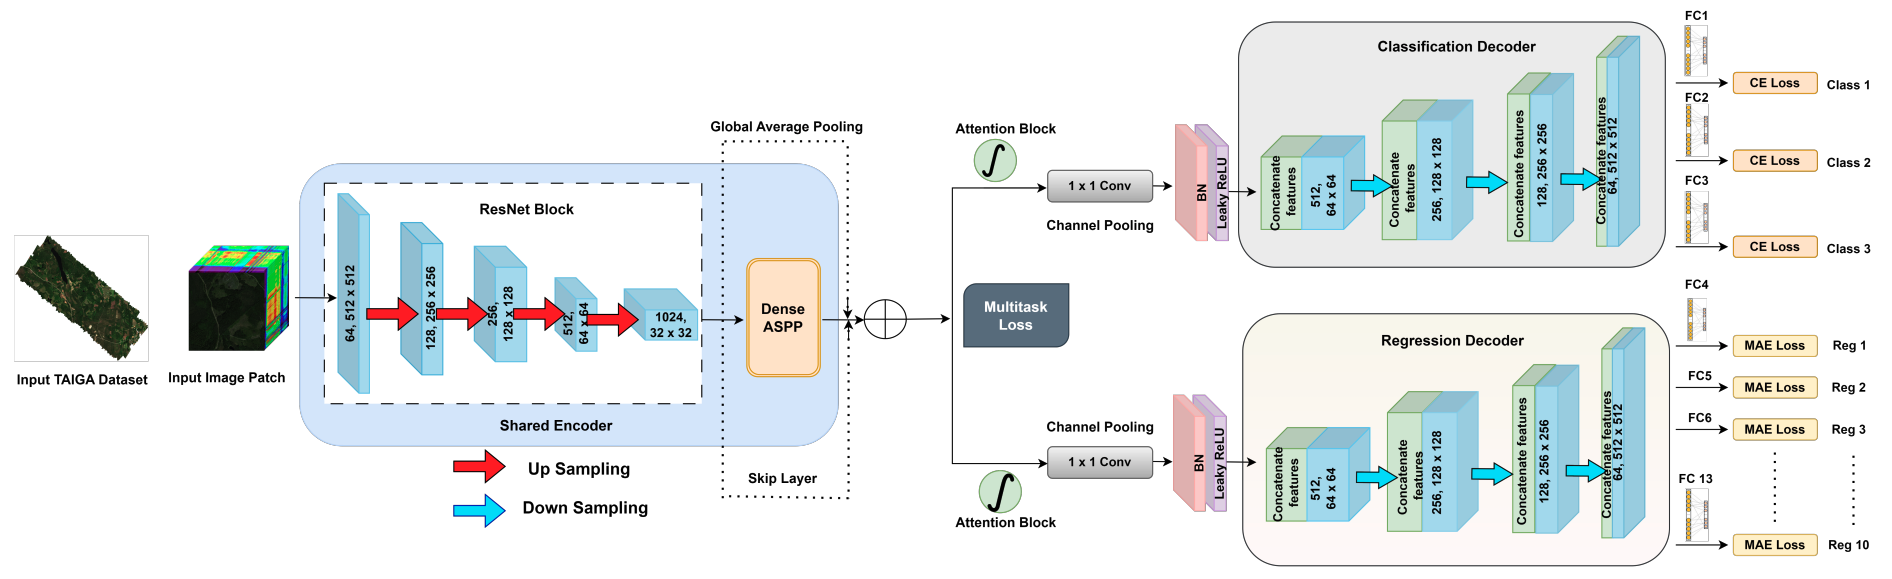
\includegraphics[width=0.95\textwidth]{img/mtl-rs-model.png}
\caption{Framework of the proposed multitask deep learning model for classification and regression of hyperspectral images. The architecture uses a shared encoder with ResNet and Dense ASPP, spectral-spatial attention blocks, and task-specific decoders. Each output has its own loss criterion: Cross-Entropy (CE) for classification and Mean Absolute Error (MAE) for regression. Adapted from \cite{chhapariya_multitask_2024}.}
\label{fig:mtl-rs-model}
\end{figure}

\cite{mottus_taiga_2022} presented TAIGA, a novel dataset for multitask learning of continuous and categorical forest variables from hyperspectral imagery. The dataset contains over 70 million labeled pixels with both continuous variables (tree height, stem volume, basal area) and categorical variables (tree species, forest type) derived from forest inventory data. They established baseline results using multitask models, showing that joint learning of continuous and categorical forest attributes improves prediction accuracy for both types of variables. The dataset enables investigation of how different forest parameters relate to each other through shared spectral signatures.

\cite{la_rosa_multi-task_2021} proposed a multi-task fully convolutional network for tree species mapping in dense forests using small training hyperspectral data. Their approach is particularly relevant for this thesis because it addresses the challenge of limited training data through multitask learning. The model implements a partial loss function that enables dense tree semantic labeling from sparse polygon-level annotations, and introduces a distance regression complementary task that enforces tree crown boundary constraints. By jointly learning species classification and distance-to-boundary regression, the model achieves 88.63\% average user accuracy and 88.59\% average producer accuracy for tree species classification in tropical forests. This demonstrates that auxiliary geometric tasks can substantially improve classification performance, similar to how TreeSatAI uses small patches for training. The key insight is that the complementary task provides additional supervision that helps the model learn better features for the primary species classification task, even when labeled data is limited.

\subsubsection{Motivation for Forest Parameter Extraction}

The application of multitask learning to forest parameter extraction from SAR is motivated by the physical relationships among forest attributes. Tree species identity influences growth patterns, wood density, and maximum attainable height. A spruce tree develops differently from an oak tree, and knowing the species provides prior information about expected height ranges. Canopy height correlates with stand age while also providing geometric information relevant to species discrimination. The height profile, crown shape, and canopy texture differ among species in ways that complement textural differences visible in SAR backscatter. By training a single model to predict species and height jointly, the shared encoder can learn features that capture these biophysical relationships, potentially improving predictions for both tasks.

However, multitask learning does not always improve performance. Sometimes it actually degrades results, a phenomenon known as \textit{negative transfer}. This occurs when tasks interfere with each other during training instead of helping each other. \cite{lyu_deep_2025} discuss negative transfer in the context of domain adaptation for remote sensing, noting that when source and target domains have conflicting feature distributions, transferring knowledge can degrade performance rather than improve it. The same principle applies to multitask learning. When tasks require conflicting representations in the shared encoder, joint training can hurt both tasks compared to training them separately.

For forest parameter extraction, species classification and height estimation appear related through the biophysical properties of trees, but they differ fundamentally in nature. One is a discrete classification problem, the other a continuous regression. The central question is whether these tasks share enough underlying structure to benefit from joint learning, or whether their different objectives create conflicting gradient signals that interfere with optimization. The classification task pushes the shared encoder to learn discriminative boundaries between species, which may help or hurt the regression task that needs smooth, continuous representations of height. When tasks compete for the limited capacity of the shared encoder, the model might end up performing both tasks worse than if they were learned separately.

Understanding when and why negative transfer occurs is crucial for designing effective multitask architectures. The gradient cosine similarity between tasks provides one way to detect conflicts. When gradients from different tasks point in opposite directions (negative cosine similarity), they are actively working against each other. Task balancing strategies, architectural choices about what to share, and careful monitoring of per-task performance during training all play a role in avoiding negative transfer.

Most existing multitask remote sensing studies leverage optical or hyperspectral imagery, either alone or in combination with SAR. This gap presents an opportunity to investigate whether the structural information encoded in SAR backscatter is sufficient to support multitask learning for forest attributes, whether negative transfer occurs when combining classification and regression from radar data, and how different parameter sharing strategies affect performance when working with radar data alone.

\section{Dataset Availability in Forest Monitoring}
\label{sec:datasets}

The development of deep learning models for forest monitoring is constrained by data availability. Unlike natural image datasets which contain millions of labeled examples, remote sensing datasets for forest applications are typically smaller and more specialized. This scarcity arises from the cost and difficulty of collecting ground-truth labels, as forest inventory measurements require trained personnel and often involve accessing remote locations.

Existing benchmark datasets for forest remote sensing tend to focus on single tasks. Some datasets provide multi-sensor imagery with species labels but do not include annotations for canopy height. Others offer LiDAR-derived height information but lack species-level labels, or cover only small geographic areas. This fragmentation means that a model trained for species classification on one dataset cannot easily incorporate height predictions from another, as the spatial locations, sensor configurations, and forest types differ.

\begin{table}[htbp]
\centering
\caption{Comparison of Forest Monitoring Datasets}
\label{tab:datasets}
\small
\begin{tabular}{lcccccccc}
\hline
\textbf{Dataset} & \textbf{S1} & \textbf{Species} & \textbf{Biomass} & \textbf{Height} & \textbf{GEDI} & \textbf{Location} & \textbf{Year} \\
\hline
FoMo-Bench & \checkmark & \checkmark & \checkmark & \checkmark & & Multiple & 2024 \\
BioMassters & \checkmark & & \checkmark & & & Finland & 2023 \\
TreeSatAI & \checkmark & \checkmark & & & \checkmark & Germany & 2023 \\
TomoSense & & \checkmark & \checkmark & \checkmark & & Germany & 2023 \\
I-MAESTRO & & \checkmark & & \checkmark & & France, etc. & 2023 \\
BAMFOREST & \checkmark & & & \checkmark & \checkmark & Germany & 2024 \\
NEON & & \checkmark & \checkmark & \checkmark & \checkmark & USA & 2021 \\
Afri-SAR & \checkmark & \checkmark & \checkmark & \checkmark & & Gabon & 2018 \\
TropiSAR & & & \checkmark & \checkmark & & Fr. Guiana & 2018 \\
AfriSAR (Full) & & \checkmark & \checkmark & \checkmark & & Gabon & 2018 \\
\hline
\end{tabular}
\end{table}

The TreeSatAI Benchmark Archive represents a notable contribution to this landscape. It provides over 50{,}000 image triplets (aerial, Sentinel-1, Sentinel-2) with labels for 20 European tree species derived from forest administration data in Lower Saxony, Germany. The dataset has enabled significant research on multi-sensor tree species classification using both traditional machine learning and deep learning methods. However, TreeSatAI focuses on species classification and does not include annotations for canopy height or other structural parameters, limiting its direct applicability for multitask learning research that combines classification and regression objectives. For canopy height specifically, several global and regional products have been developed. ~\cite{potapov_mapping_2021} produced a 30~m resolution global forest height map using GEDI and Landsat data with tree ensemble methods, achieving mean error of 9.1~m. ~\cite{lang_high-resolution_2023} improved upon this with a 10~m resolution global canopy height model using deep learning on Sentinel-2 and GEDI data, achieving RMSE of 7.9~m. More recently, ~\cite{tolan_very_2024} achieved sub-meter resolution canopy height maps using DiNOv2 models with high-resolution Maxar imagery and airborne LiDAR. These products provide potential sources for deriving height labels to extend species classification datasets. This situation motivates the exploration of dataset extension strategies. If canopy height estimates can be derived from auxiliary sources such as global canopy height products, regional LiDAR surveys, or forest inventory statistics, it becomes possible to augment existing species classification datasets for multitask learning. The quality and reliability of these derived labels, and their impact on multitask model performance, are important questions. By investigating how TreeSatAI can be extended with height information, this research aims to establish practical pathways for creating multitask-ready resources.

\subsubsection{Additional Datasets.} 
Several other datasets were reviewed but not selected for this study. The iMAESTRO dataset~\cite{aussenac_diameter_2023} is derived from Airborne Laser Scanning measurements combined with field inventory data and vegetation maps. It provides tree-level records with species identity, diameter, height, and position for over 42 million individual trees across three European forest regions (Bauges, Milicz, Sneznik). The dataset enables generation of pixel-level labels for genus segmentation, canopy height, and biomass. From a multitask learning perspective, the complete co-registration of all target variables makes it suitable for investigating whether biomass and height predictions benefit from shared representations, and whether genus segmentation provides useful features for structural estimation. However, it does not include Sentinel-1 SAR imagery directly, requiring separate acquisition and processing of SAR data. BioMassters \cite{andrea_nascetti_biomassters_nodate} provides Sentinel-1/2 imagery with biomass labels for Finnish forests, but does not include separate species annotations and the released GeoTIFFs have geolocation metadata removed. BAMFOREST \cite{troles_bamforests_2024} offers UAV-based tree crown segmentation with height information, though species labels are provided as broad categories (coniferous/broadleaf) rather than specific species. TomoSense \cite{tebaldini_tomosense_2023} contains multi-frequency tomographic SAR with species, biomass, and height labels, but the 3D tomographic cube format differs from conventional 2D image inputs, and existing implementations adapting this data for standard encoder-decoder architectures are limited. NEON \cite{weinstein_remote_2021} covers 47 US sites with species, biomass, and height measurements, though field surveys are conducted in 20$\times$20~m subplots within larger plots, resulting in incomplete spatial coverage relative to the airborne imagery. TropiSAR \cite{dubois-fernandez_tropisar_2012} and AfriSAR \cite{fatoyinbo_nasa_2021} provide tropical forest measurements with biomass and height at plot level, but species labels are either absent (TropiSAR) or sparsely distributed at individual tree positions within discrete plots (AfriSAR). FoMo-Bench \cite{bountos_fomo_2025} aggregates 15 datasets for forest monitoring tasks, though the heterogeneous sources have varying acquisition dates, resolutions, and annotation protocols, and published work demonstrating its use for joint species-height prediction specifically is limited.

\subsubsection{Motivation for Dataset Extension.}
The decision to extend TreeSatAI rather than create an entirely new dataset was driven by several practical considerations. First, TreeSatAI already provides high-quality species labels from official forest administration records, eliminating the need for costly field campaigns or manual annotation. Second, the benchmark's spatially distributed sampling across Lower Saxony ensures representation of diverse forest types and management practices. Third, the availability of official German LiDAR-derived elevation products (DTM and DSM) from the same geographic region enables accurate height label generation without requiring new airborne surveys.

From a scientific perspective, adding height information to TreeSatAI addresses a key gap in SAR-based forest monitoring research. While optical remote sensing benefits from well-established relationships between spectral signatures and both species composition and canopy structure, SAR backscatter patterns are more complex and less studied for joint species-height prediction. By creating a dataset that pairs SAR imagery with both categorical (species) and continuous (height) labels, this research enables investigation of whether these tasks share beneficial representations in the SAR domain, potentially improving performance on both tasks through multitask learning.
